\documentclass[a4paper, 12pt]{article}

\usepackage[utf8]{inputenc}
\usepackage[french]{babel}
\usepackage[T1]{fontenc}
\usepackage{geometry}
\usepackage{amsmath}
\usepackage{amsfonts}
\usepackage{amssymb}
\usepackage{adjustbox}
\usepackage{rotating}
\usepackage{graphicx}
\usepackage{wrapfig}
\usepackage{lscape}
\usepackage{epstopdf}
\usepackage{pdflscape}
\usepackage{titles}
\usepackage{float}
\usepackage{uniquecounter}
\usepackage{hyperref}
\usepackage{enumitem}
\usepackage[table]{xcolor}
\usepackage{array}
\usepackage{bookmark}
\usepackage{booktabs}
\usepackage{pifont}
\usepackage{colortbl}
\usepackage{multirow}
\usepackage{longtable}
\usepackage{adjustbox}
\usepackage{ltablex, array}
\usepackage{tikz}
\usepackage{fontawesome5}
\usepackage{utfsym}
\usepackage{fourier}
\usepackage{pdfpages}
\usepackage{lscape}
\usepackage{tabularx}

\hypersetup{
    colorlinks,
    citecolor=black,
    filecolor=black,
    linkcolor=black,
    urlcolor=black
}

\definecolor{grey_prestation}{RGB}{238, 240, 255}

\title{Cahier des charges\\
La Socketterie}
\author{Entreprise Webatom}
\date{09/2024}

\setlength{\footskip}{20pt}
\setlength\parindent{0pt}
\begin{document}
\maketitle
\begin{figure}[H]
    \centering
    
\includegraphics[scale=1]{La socketterie.png}
\end{figure}
\clearpage

\tableofcontents
\newpage
\section{L'entreprise}
\subsection{Présentation de l'entreprise}
La Socketterie est une entreprise de tricot et de vente de chaussettes dépareillées dans une boutique physique fondée en 2019 à Nice en France.\\
Les employés du magasin accueillent et accompagnent les consommateurs avec sincérité et bienveillance. L'ambiance du magasin est chaleureuse.\\
En outre, l'entreprise prône la qualité de ses produits dont une bonne durabilité.
\subsection{Valeurs de l'entreprise}
L'entreprise dispose de valeurs fortes telles que l'entraide, la solidarité, l'empathie et l'engagement. 
En conséquences, elle reverse 1\% de son chiffre d'affaires à une association d'aide à l'employabilité des personnes atteintes de trisomie. (présente chaque 21 mars à la journée mondiale de la trisomie).\\

\subsection{Description des produits et services}
L'entreprise tricote elle-même des chaussettes dépareillées de couleurs souvent vives. Composées de laine ou de soie, tous les matériaux sont 100\% français. La qualité des produits leur permet de rester durables pendant 3 à 5 ans.\\
Ces chaussettes sont actuellement disponibles à l'achat dans le magasin physique.
\subsection{Public cible}
La population ciblée est jeune : entre 20 et 35 ans. Leurs moyens les plus communs pour s'informer sont les réseaux sociaux et les sites Web.\\
Par ailleurs, les tendances du moment montrent que cette tranche d'âge est plus encline à consommer ce type de produit plutôt que des produits classiques.
\subsection{Analyse des concurrents principaux}
\subsubsection{"Les trésors de Chloé"}
\url{https://lestresorsdechloe.com/}\\
Type : site e-commerce\\
Plugins : Jquery, OWL Carousel\\
Charte graphique :
\begin{figure}[H]
    \centering
    
\includegraphics[scale=0.4]{theme_chloe.jpeg}
\end{figure}
Moyen de paiement : paiement en ligne propulsé par l'API SystemPay.\\
Points forts :
\begin{itemize}
    \item Interface claire et ergonomique.
    \item Bandeau d'actualités défilants attirant le regard.
    \item Menu simple et visible.
\end{itemize}
Points faibles :
\begin{itemize}
    \item Retour à la page d'accueil peu clair.
    \item Icones de panier, connexion et recherche pas très visibles.
    \item Quelques bugs graphiques.
\end{itemize}
\subsubsection{"La Chaussette Française"}
\url{https://boutique.la-chaussette-francaise.com/}\\
Type : chaîne de magasin avec adresse physique à Nice et site e-commerce.\\
Plugins : WordPress et Jquery.\\
Charte graphique :
\begin{figure}[H]
    \centering
    
\includegraphics[scale=0.4]{theme_chaussette_francaise.jpeg}
\end{figure}
Moyen de paiement : Visa, Eurocard/Mastercard, Paypal, par chèque ou par virement bancaire.\\
Points forts :
\begin{itemize}
    \item Site très dynamique.
    \item Produits très bien mis en avant.
    \item Site épuré et conscis.
\end{itemize}
Points faibles :
\begin{itemize}
    \item Site mal référencé.
    \item Boutons utilitaires peu visibles.
    \item Le design et la charte graphique ne sont pas mémorables. Le Site ressemble trop aux sites e-commerces standards.
\end{itemize}
\newpage
\section{Le projet}
\subsection{Objectifs du site}
\subsubsection{Objectifs qualitatifs}
\begin{itemize}
    \item Permettre l'achat de chaussettes en ligne.
    \item Donner plus de visibilité à l'entreprise.
    \item Gérer les stocks de l'entreprise.
\end{itemize}
\subsubsection{Objectifs quantitatifs}
\begin{itemize}
    \item Permettre de récolter des avis sur les produits et l'entreprise.
    \item Augmenter les ventes.
\end{itemize}
\subsection{Charte graphique}
\subsubsection{Identité visuelle}
Le logo est le suivant :
\begin{figure}[H]
    \centering
    
\includegraphics[scale=0.6]{La socketterie.png}
\end{figure}
A la demande du client, la palette de couleurs sera la suivante :
\begin{figure}[H]
    \centering
    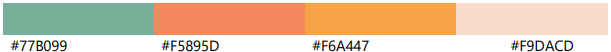
\includegraphics[scale=1]{palette_couleur.png}
\end{figure}
En utilisant la police Stadio Now Display\\ (\url{https://fontsfree.net/stadio-now-trial-display-bold-font-download.html})\\
Le client demande une alternance des couleurs sur le site pour reproduire le visuel d'une chaussette comme sur leur logo. De plus, la page Web devrait être assez épurée pour s'adapter aux mobiles ainsi que présenter un carousel d'images présentant les employés et leur méthode de tricot dans un onglet présentation.
\subsubsection{Ergonomie}
Le logo et les menus doivent être clairement visibles. Les consommateurs devraient facilement rester informés des nouveautés.\\
Le client apprécie la présence d'un bandeau d'information sur les promotions sur le site suivant : \url{https://lestresorsdechloe.com/}
\subsection{Maquette}
La page d'accueil se doit donc d'être plutôt épurée, agréable sur mobile et présenter brièvement les nouveautés et l'entreprise. L'intégration des couleurs devra se faire en prenant en compte l'aspect chaleureux de l'entreprise.\\
Voici une proposition de maquette pour la page d'accueil reprenant l'identité visuelle demandée :
\begin{figure}[H]
    \centering
    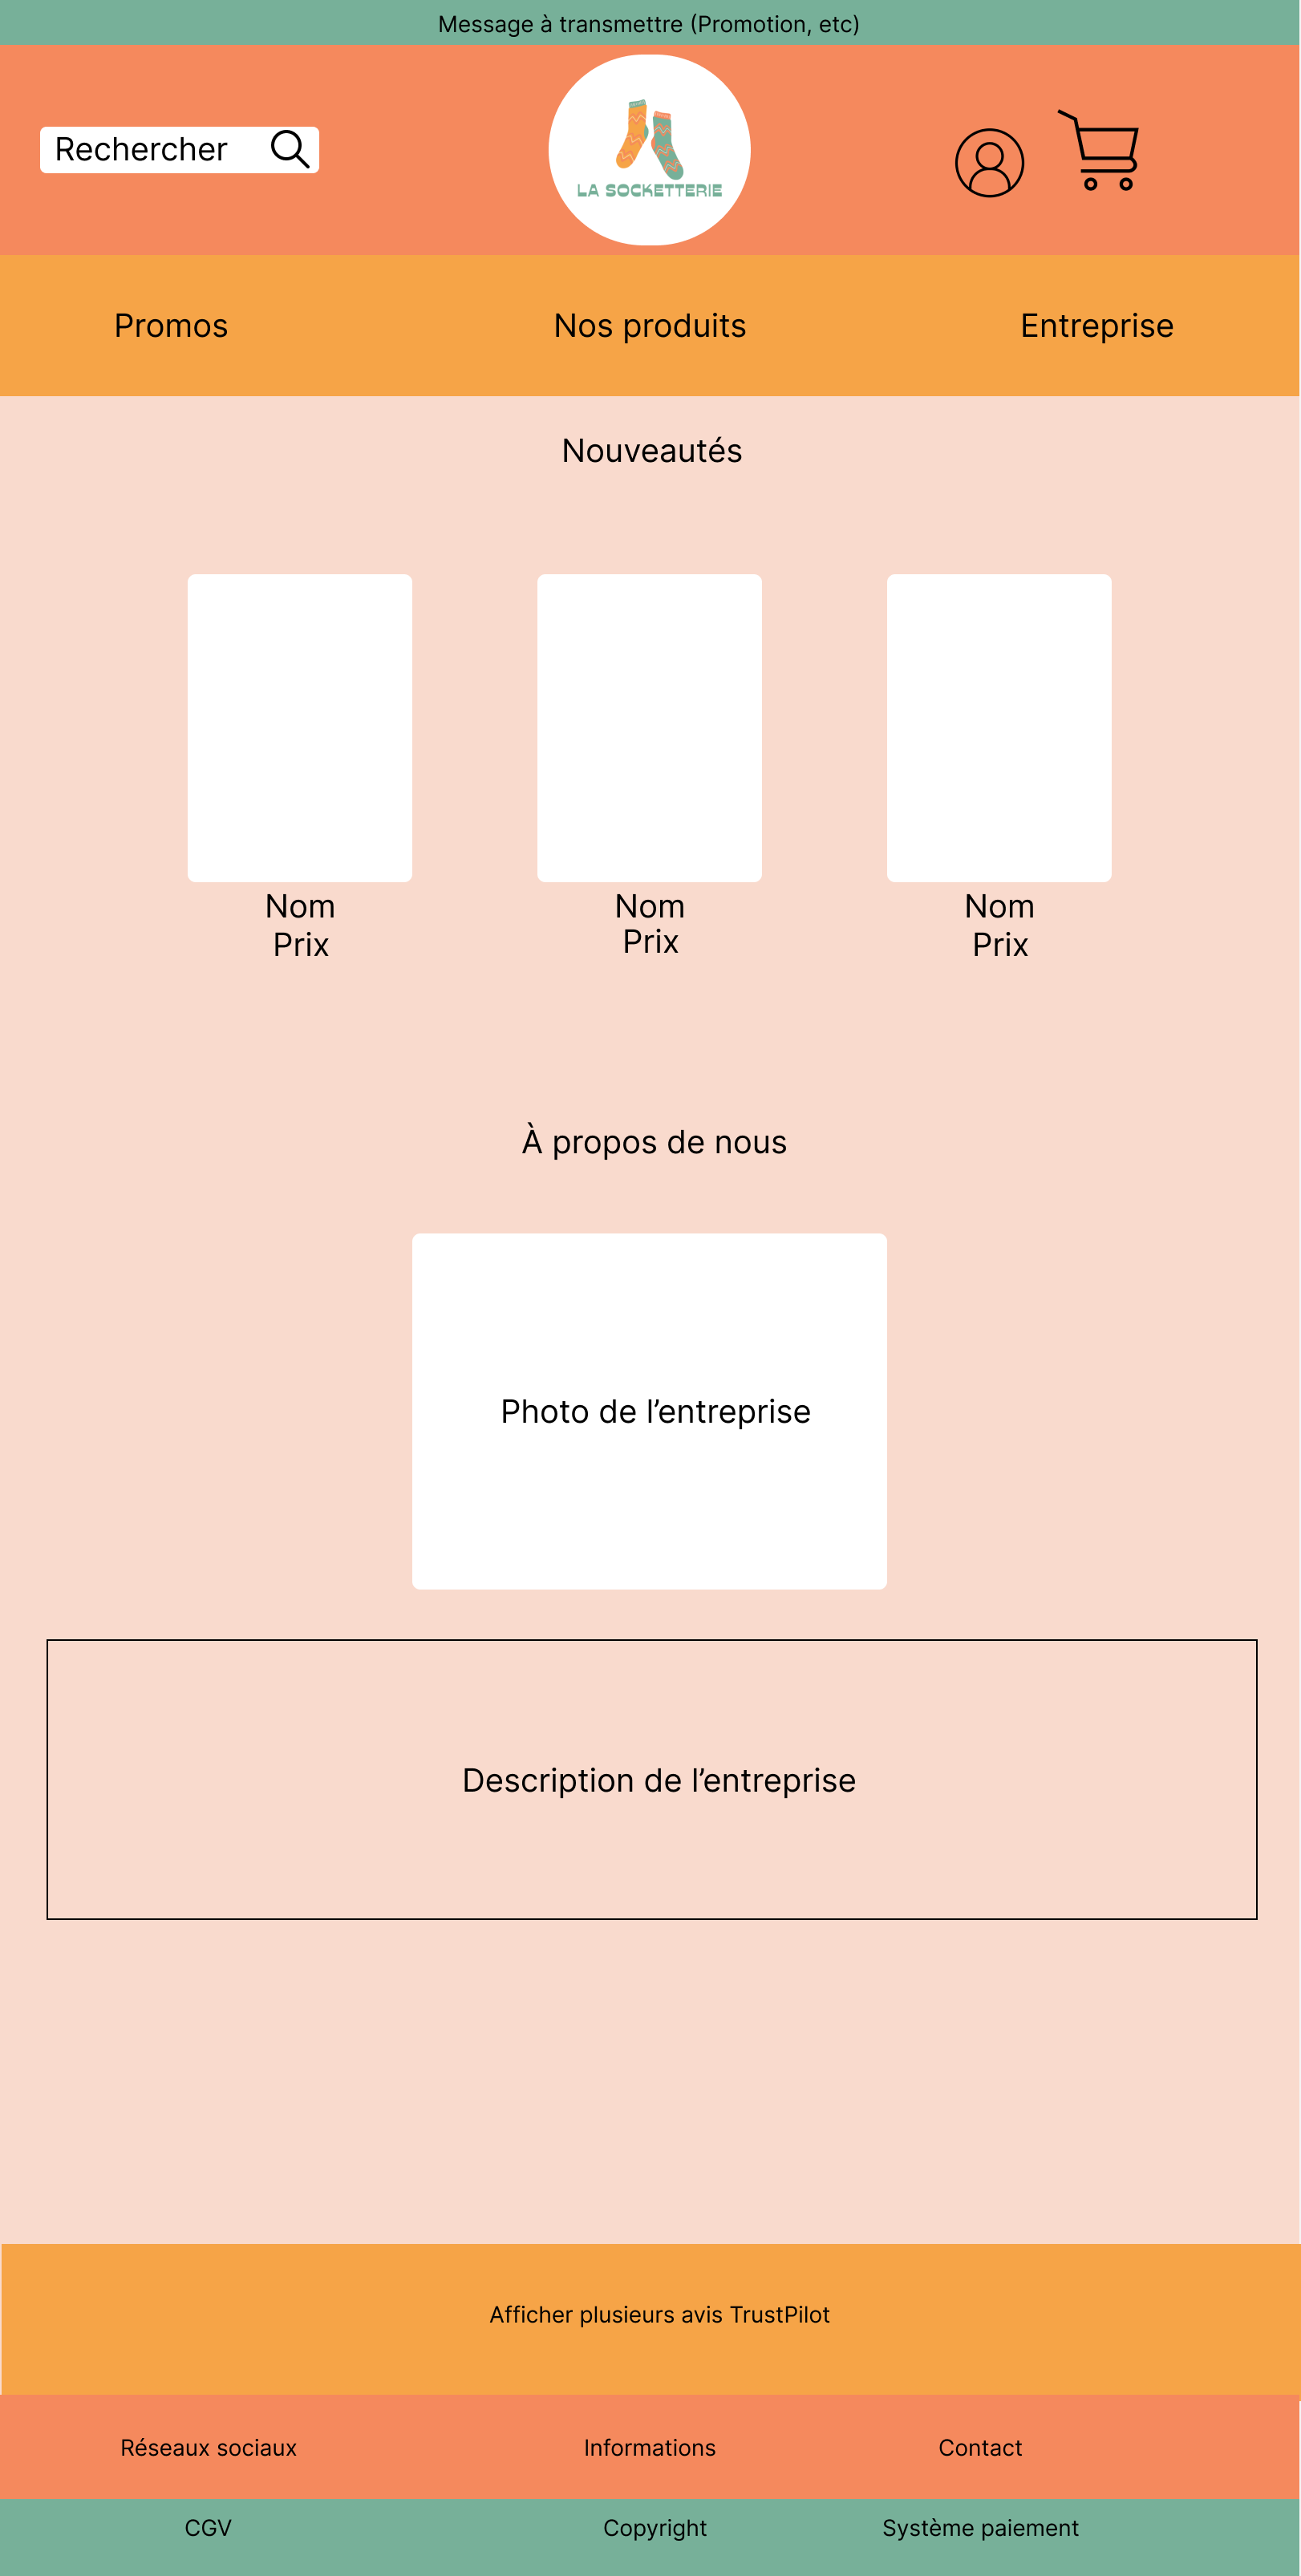
\includegraphics[scale=0.32]{Untitled@2x.png}
\end{figure}
\subsection{Arborescence du site}
La page d'accueil devrait donc présenter trois onglets principaux :
\begin{itemize}
    \item Un onglet pour s'informer des promotions.
    \item Un onglet pour consulter le catalogue des produits.
    \item Un onglet pour présenter l'entreprise.
\end{itemize}
\begin{figure}[H]
    \centering
    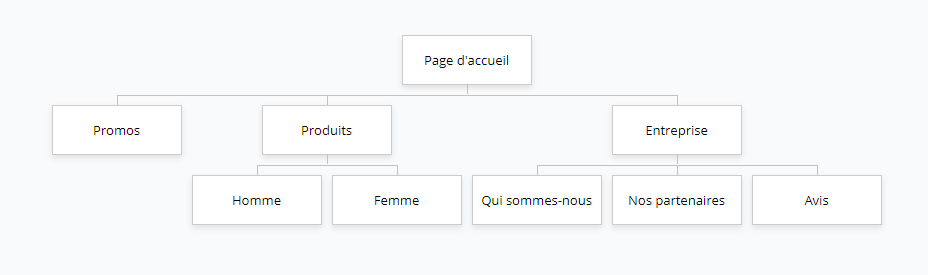
\includegraphics[scale=0.7]{arborescence.png}
\end{figure}
\subsection{Spécificités}
\begin{itemize}
    \item Dans le but de réduire le coût de production et pour permettre de réduire le temps de production, l'API SumUp sera utilisé.
    \item Prendre en compte l'intégration de photos et/ou de vidéos possibles concernant la fabrication des produits ou autre ; notamment dans le carousel de présentation de l'entreprise.
    \item Le site Web devra s'adapter aux mobiles.
\end{itemize}

\section{Options de développement}
\subsection{Contraintes techniques}
\begin{itemize}
    \item Site hébergé chez OVH.
    \item Respect de la RGPD.
    \item Création et formation à l'utilisation d'une partie back-office.
    \item Création d'une zone d'avis utilisant TrustPilot.
\end{itemize}
\subsection{Périmètre du projet}
Le magasin étant proche de l'Italie, l'intégrations de plugins pour changer la langue du site en italien ou anglais est à prévoir. Le plugin Weglot sera utilisé.\\

Comme dit précedemment, le public cible impose que le site soit agréable sur mobile.\\

L'API SumUp possède directement un système de paiement qui sera utilisé.\\

Les livraisons seront gérées par l'entreprise Colissimo. L'installation du plugin Colissimo Entreprise sera nécessaire.\\

La gestion du catalogue est directement proposée par l'API SumUp dans l'espace dédiée à cet effet.
\newpage
\section{Livrables}
\subsection{Qui sommes-nous ?}
Jeune entreprise créé en 2024, nous mettons un point d'honneur à satisfaire les clients et proposer des solutions à moindre coût.
\subsection{Prestations}
\includepdf[pages=-]{Facture N°20240900001 - La Socketterie.pdf}
\begin{landscape}
    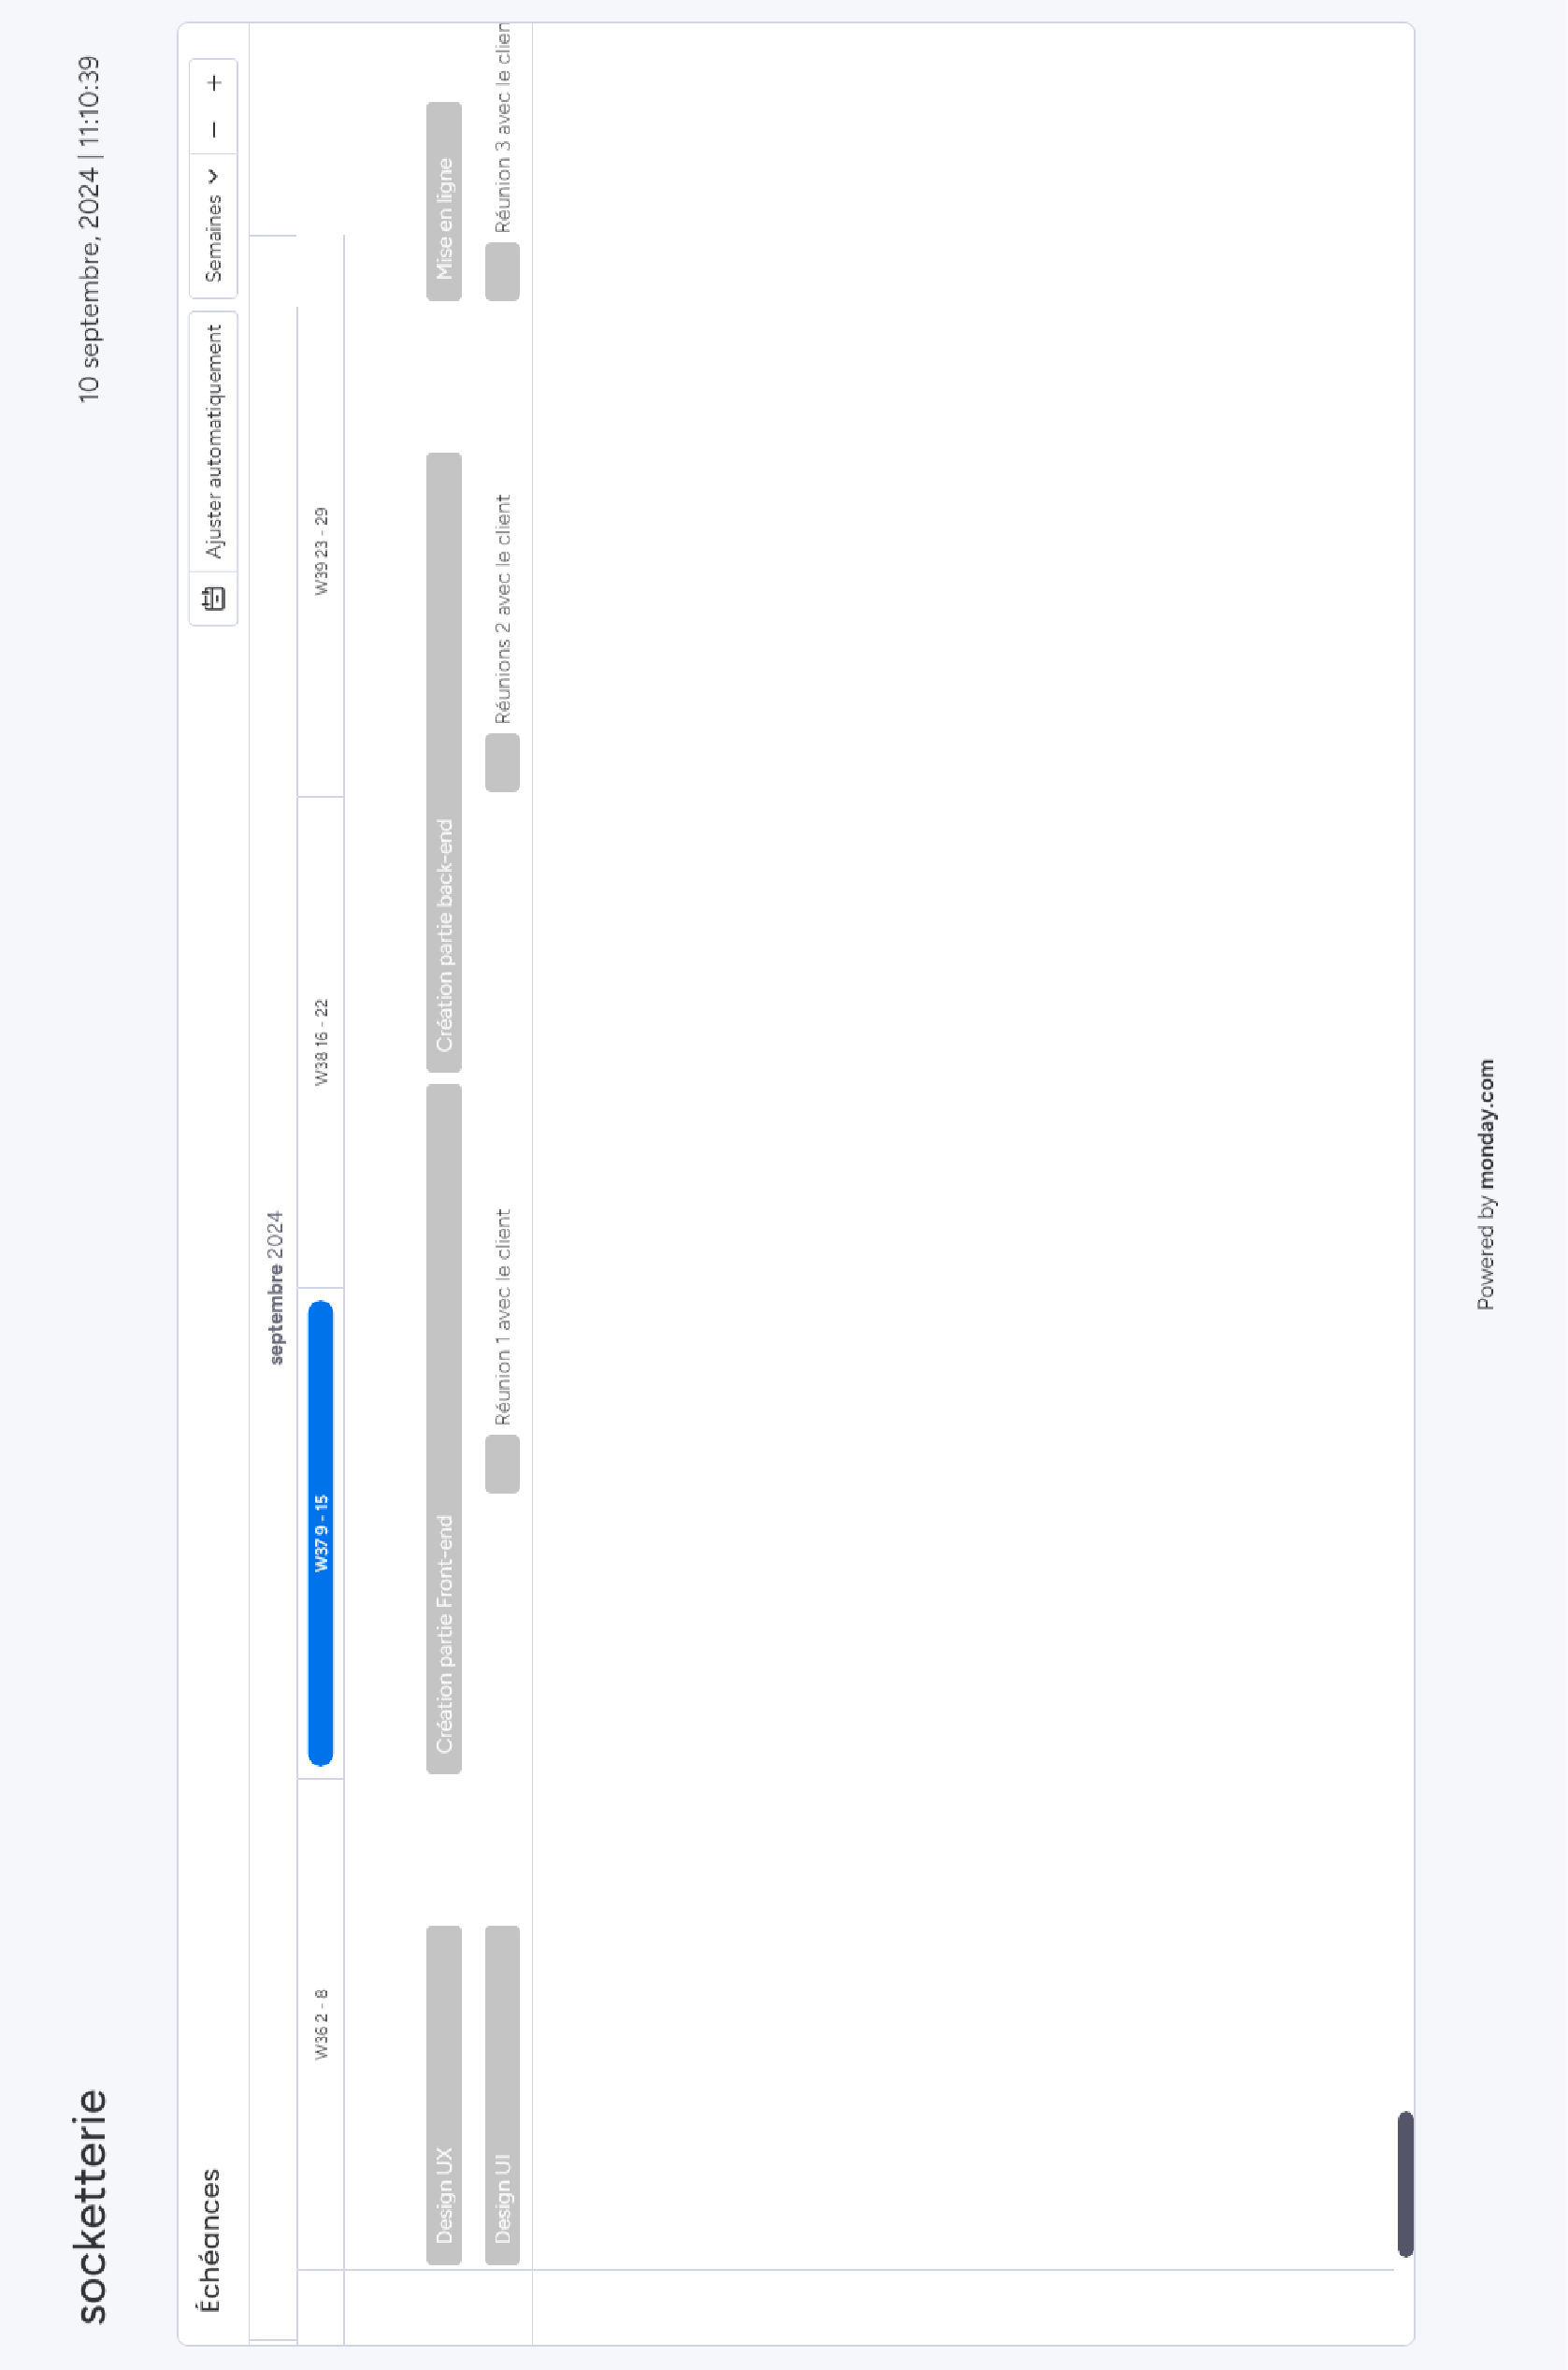
\includepdf[pages=-, pagecommand=\subsection{Planning}]{socketterie_rotated.pdf}
\end{landscape}
\section{Conclusion}
\begin{tabularx}{\linewidth}{|l|X|}
\hline
\multicolumn{2}{|c|}{Charte graphique}\\
\hline
Logo & 
\includegraphics[scale=0.3]{La socketterie.png}\\
\hline
Palette de couleurs & 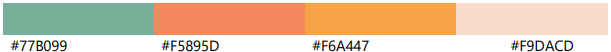
\includegraphics[scale=0.6]{palette_couleur.png}\\
\hline
Police d'écriture & Stadio Now Display (\url{https://fontsfree.net/stadio-now-trial-display-bol
html})\\
\hline
Caractéristiques & Design épuré pour mobile. Carousel d'images de l'entreprise.\\
\hline
\multicolumn{2}{c}{}\\
\hline
\multicolumn{2}{|c|}{Options de développement}\\
\hline
APIs & SumUp\\
\hline
Hébergeur & OVH\\
\hline
Back-Office ? & Oui, gestion de catalogue via SumUp\\
\hline
Multilingue & Français, Italien et Anglais. Plugin Weglot\\
\hline
Livraison & Colissimo. Plugin Colissimo Entreprise\\
\hline
Système de paiement & SumUp\\
\hline
Avis & TrustPilot\\
\hline
\multicolumn{2}{c}{}\\
\hline
\multicolumn{2}{|c|}{Précisions}\\
\hline
Cible & jeune : entre 20 et 35 ans\\
\hline
\end{tabularx}
\end{document}